\documentclass{article}

\PassOptionsToPackage{numbers, compress}{natbib}

% \usepackage{neurips_2024}
\usepackage[preprint]{neurips_2024}
% \usepackage[final]{neurips_2024}
% \usepackage[nonatbib]{neurips_2024}


\usepackage[utf8]{inputenc} % allow utf-8 input
\usepackage[T1]{fontenc}    % use 8-bit T1 fonts
\usepackage{hyperref}       % hyperlinks
\usepackage{url}            % simple URL typesetting
\usepackage{booktabs}       % professional-quality tables
\usepackage{amsfonts}       % blackboard math symbols
\usepackage{nicefrac}       % compact symbols for 1/2, etc.
\usepackage{microtype}      % microtypography
\usepackage{xcolor}         % colors
\usepackage{graphicx}       % for including graphics
\usepackage{amsmath}


\title{EE245 Project Final Report \\ \large A Study on Reinforcement Learning for Parking: Vision/Radar/LiDAR Sensing}

\author{
  Kunyi Yu\\
  Student ID: 862548836 \\
  % Department of Computer Science and Engineering\\
  University of California, Riverside\\
  Riverside, CA 92521\\
  kyu135@ucr.edu
}

\begin{document}

\maketitle

\begin{abstract}
  5\% The abstract content \dots
\end{abstract}

% 7-8 pages excluding references
% Abstract (5%)
% Introduction (15%)
% Related Work (15%)
% Method (30%)
% Experiments (30%)
% Conclusion (5%).

\section{Introduction 15\%}

Traffic accidents caused by human judgment errors remain a leading cause of fatalities worldwide. However, the rapid development of autonomous driving technologies holds promise for significantly reducing such incidents. In December 2024, the author visited the Bay Area and observed a growing presence of autonomous vehicles (AVs) on the road, either undergoing testing or already in commercial operation. Waymo, one of the industry pioneers, has been operating a fleet of AVs in San Francisco since August 2021. On the other hand, unlike Waymo’s radar-based approach, Tesla’s Full Self-Driving (FSD) system relies primarily on vision-based sensing. Tesla’s commercial success demonstrates that a camera-only solution can be viable for autonomous driving.

Sensing modality, like vision, Radar or LiDAR, are widely researched and adopted in the industry, each with its own advantages and limitations. A 2024 news report \cite{news2024} highlighted an incident where Waymo’s AVs were excessively honking in a San Francisco parking lot, disturbing nearby residents multiple times at night. The issue was reportedly caused by interference from other vehicles, leading to a deadlock scenario—a common challenge in multi-agent systems. This also underscores the complexity and importance of autonomous parking as a research topic.

Thus, the modality of sensing is crucial for autonomous driving, especially in complex environments like parking lots where dense traffic and pedestrians could lead to problems such as deadlocks and security concerns. Reasonable solutions could be combined with different sensing modalities or dynamically switching between them to enhance the robustness of the system. Therefore, this project aims to explore the effectiveness of different sensing modalities in various parking scenarios by horizontally comparing the performance of several reinforcement learning (RL) algorithms. 

In the rest of this report, Section \ref{sec:related_work} reviews related work in the the application of RL algorithms in autonomous parking and some common sensing modalities. Section \ref{sec:methodology} describes the methodology, including task definition, environment setup, RL algorithms, observation modalities, reward function and training settings. Section \ref{sec:experiments} presents the experimental results, including the performance comparison and findings. Finally, Section \ref{sec:conclusion} includes summary, contributions, and future work.

\newpage

\section{Related Work 15\%}\label{sec:related_work}

This section reviews related work in the application of reinforcement learning (RL) algorithms in autonomous parking and common sensing modalities in autonomous driving. Most papers in this section are based on the \texttt{highway-env} environment \cite{highway-env}, which is the platform used in this project and also widely adopted in the autonomous driving research community.

\subsection{Reinforcement Learning in Autonomous Parking}

The \texttt{highway-env} environment \cite{highway-env} is a widely used platform (2.9k star on GitHub) for simulating autonomous driving scenarios, including parking tasks. The well written documentation and abided by OpenAI Gym API make it easy to use and extend. The environment provides multiple sensing modalities (Kinematics, GrayScale Image, LiDAR, etc.), continuous/discrete action spaces, and predefined scenarios with reward functions.

There are several papers study the autonomous parking problem directly in the \texttt{highway-env} environment. \citet{kapoor2020model} introduces a model-based RL approach that integrates neural dynamics prediction with Signal Temporal Logic (STL) guided model predictive control, applied to robotics and autonomous driving. This approach is demonstratesd on toy robotics tasks including a parking-lot scenario. The key strenth is its use of formal task specifications to helps avoid reward-shaping issues. A weakness is that it relies on a learned model and uses computationally expensive planning.

\citet{moreira2021deep}'s master's thesis proposes a deep reinforcement learning method with SAC, DDPG, and TD3 algorithms to teach a wheeled vehicle to park in confined spaces. The agents are trained in a simulated environment to follow a predefined parking trajectory. The study finds that TD3 converges fastest and achieves the most reliable policy, while SAC also learns satisfactorily but DDPG is less stable and efficient. Strengths of this work include a thorough comparison and careful designed reward function. However, the method needs to predefined the parking path manually and leaves out perception or sensing issues.

\citet{lazzaroni2023automated} presents a DRL-based agent trained in different environments (a Unity-based, highway-env, and CARLA) for low-speed parking maneuvers, achieving a 97\% success rate. The paper also uses Stable-Baselines3 \cite{stable-baselines3} toolkits for training the agents, which provides a set of reliable RL algorithm implementations. The ego-vehicle is equipped with a 360-degree LiDAR sensor, and the agent observation also includes relative target position and self velocity. Training uses PPO algorithm with MLP. Although the high success rate is impressive, the long training time (over 60M timesteps) and needs for hyperparameter tuning are drawbacks.

Note that Stable-Baselines3 \cite{stable-baselines3} is library of reliable implementations of standard deep reinforcement learning algorithms. It is not specifically designed for autonomous driving, but provides high-quality code for many algorithms (PPO, DDPG, SAC, TD3, A2C, etc.) with consistent API. There also exist some YouTube videos \citep{youtube2019,youtube2022} visulizing the training process of reverse parking and parallel parking. The former video uses a version of Rainbow DQN on raw camera images, showing that even a complex 3D task like reverse parking can be learned but missing performance metrics and robustness analysis due to the pattern of videos. The latter one utilizes a PPO-based policy using Unity3D environment. However, details on sensors (maybe also vision-based), reward function, or evaluation are not provided.

A survey paper \cite{elallid2022comprehensive} provides a comprehensive overview of RL applications in autonomous driving, not limited to only parking scenarios. With in this survey, some instances parking tasks are discussed, including a RL-guided Monte Carlo Tree Search (MCTS) algorithm research. Strengths is its comprehensive coverage of perception, planing, and control. As it is a high-level review, however, sensor modalities for parking are not included.

\subsection{Sensing Modalities in Autonomous Driving}

The operational logic of autonomous system, from a simple housekeeping robot to a complex self-driving car, can be summaryized into a foundamental loop: See, Think, Act. In this paradigm, the "See" component-perception-serves as the foundation layer upon which all subsequent capabilities are built. To meet the stringent safety and reliability demands of autonomous driving, the academic and industrial have invested significant sensing strategies: cameras (Vision), Radio Detection and Ranging (Radar), and Light Detection and Ranging (LiDAR). As no signle sensor can provide a complete and infallible representation of the environment, each sensing modality provide unique advantages and inherent limitations.

\citet{yurtsever2020survey} provides a comprehensive survey on common practices and emerging trends, including serveral sensoring technologies: vision-based sensors (monocular cameras, omnidirectional cameras, and event cameras), radar, and LiDAR (Point clouds). Firstly, \underline{vision-based sensors} have advantages in color sensing, passive sensing, and low cost due to established technology. However, their illumination sensitivity and difficulty in depth perception are significant drawbacks. \underline{Radar} sensors, on the other hand, have better long range detection, robustness to bad weather, and also low cost. However, they have lower resolution and their field of view is limited. Lastly, \underline{LiDAR} have pros in high accuracy, accuracy in depth perception, and robustness to illumination changes. However, they are expensive, heavy, and require large-scale data processing. If combing these sensors, the advantages of each sensor can be utilized. The figure \ref{fig:sensing_modalities} illustrates the pros and cons of these three sensing modalities.

\begin{figure}[h]
    \centering
    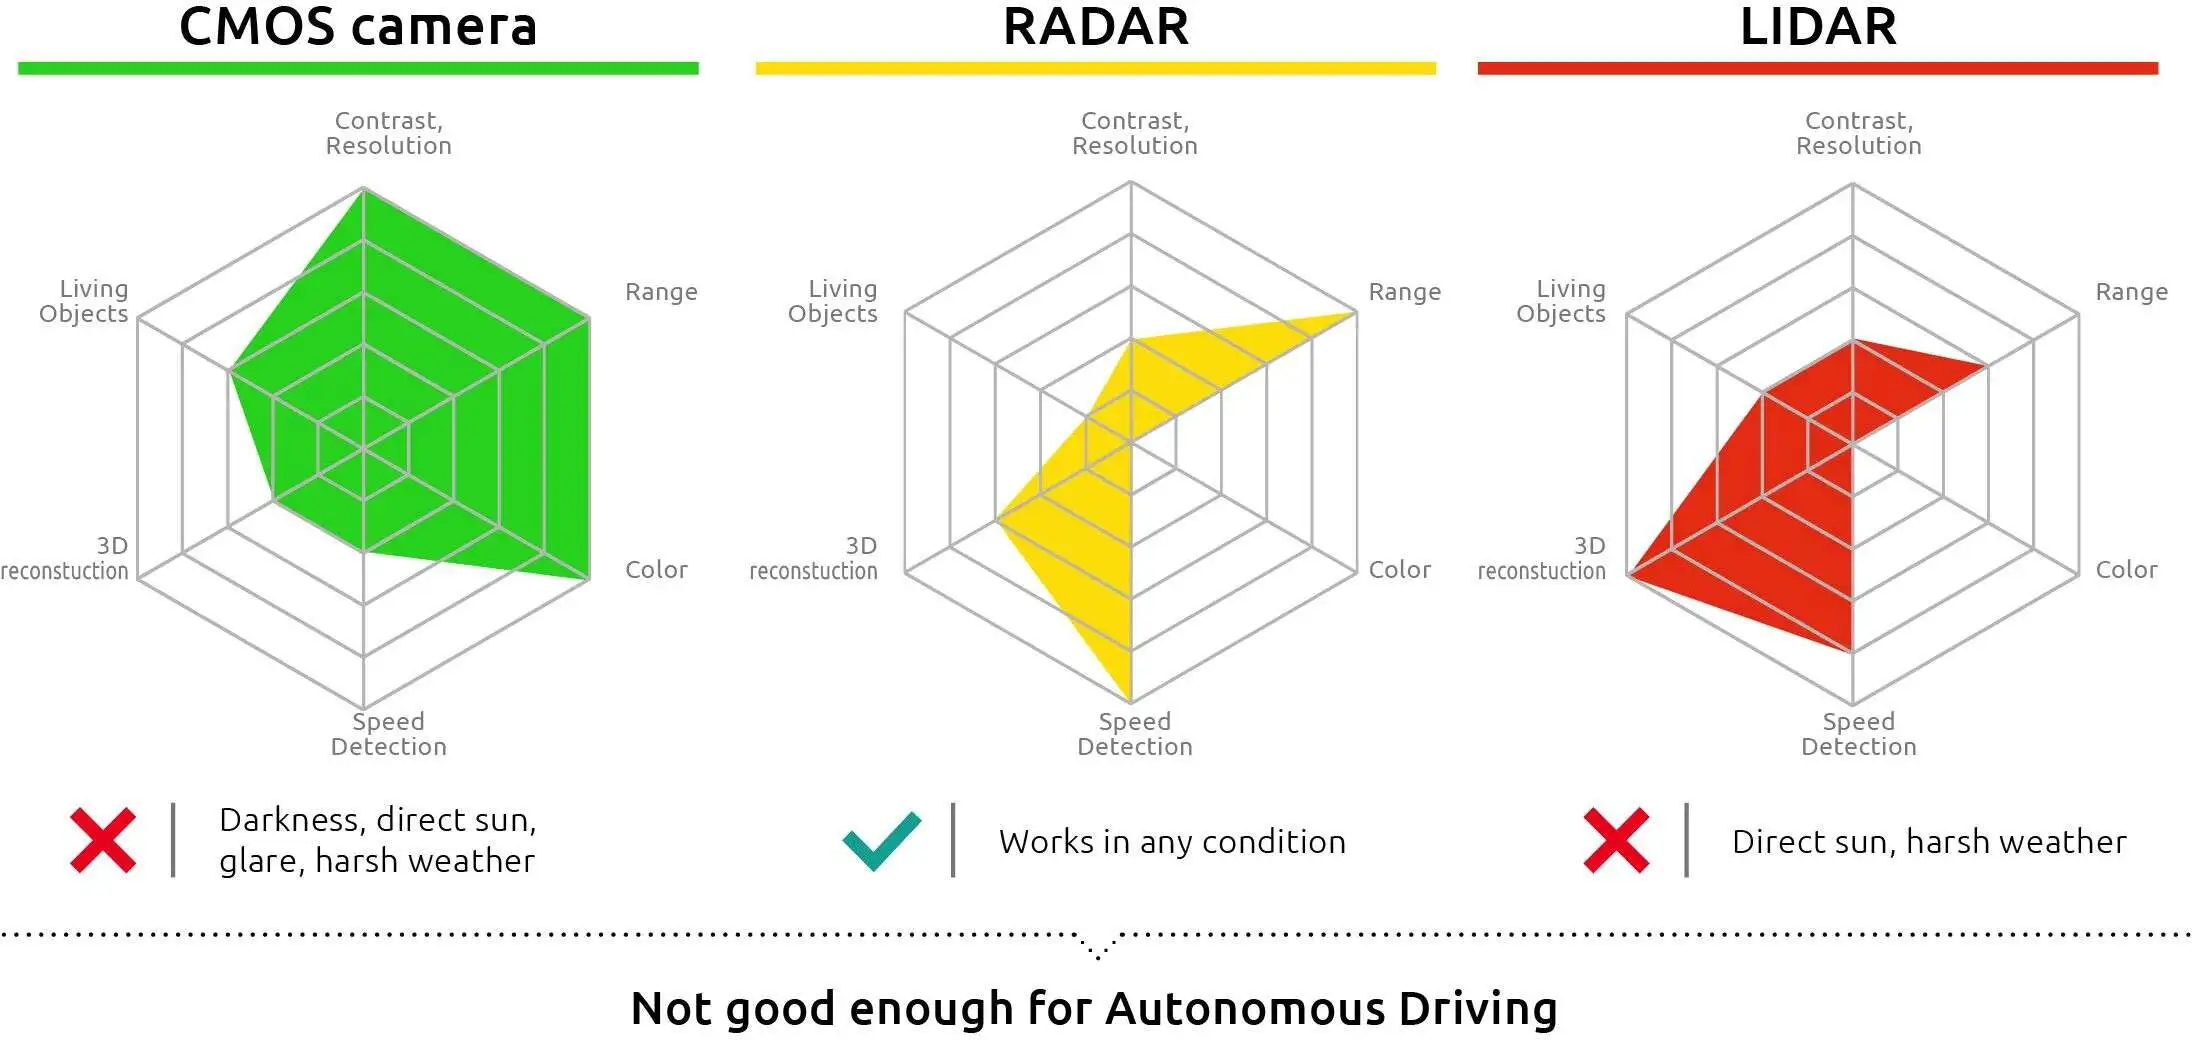
\includegraphics[width=0.8\textwidth]{./pics/3_sensors.png}
    \caption{Pros and cons of common sensing modalities in autonomous driving. (from the internet)}
    \label{fig:sensing_modalities}
\end{figure}

Some studies also explore the integration of multiple sensing modalities. \citet{pederiva2025light} alleviates the computationally demands of tranditional detecting objects by integrating Camera and LiDAR data. Their method utilizes cutting-edge Deep Learning techniques into the feature extraction process achieving a 2.39\% accuracy improvement and 10\% parameter reduction within 10 ms inference time. The lightweight and powerful model is suitable for real-time applications.

\section{Methodology 30\%}\label{sec:methodology}

This section describes the methodology of this project, including task definition, environment setup, reinforcement learning (RL) algorithms, observation, reward function and training settings.

\subsection{Task Definition and Environment Setup}

The ultimate goal of teaching a vehicle to park is to enable it to autonomously navigate and park in any real-world parking lot fast and precisely while avoiding collisions with other vehicles, obstacles, and pedestrians. For each epoch, the ego-vehicle is spawned at a random position and orientation in the parking lot, and the goal is to park it in a randomly selected parking spot. The objective function is to maximize a return $G_t = \sum_{t=0}^{T} \gamma^t r_t$, where $r_t$ is the reward at time step $t$ and $\gamma$ is the discount factor.

To abstract the task and make it suitable for RL research, the project used a simulated environment based on the \texttt{highway-env} platform \cite{highway-env} with varing other vechicles denseness to change the difficulty. In details, there will be \texttt{empty}, \texttt{normal}, and \texttt{almost-full} parking lots, which have 0, 3, and 10 other vehicles, respectively. The parking lot is a 2D continuous space with 15 spots for both north and south side as the figure \ref{fig:parking_lot} shows. The ego-vehicle is a 4-wheeled car can be controlled by fixed steering angles and acceleration. The success of parking is defined as the ego-vehicle being within a certain distance to the parking spot without angle requirement (but will be penalized in the reward function).

\begin{figure}[h]
    \centering
    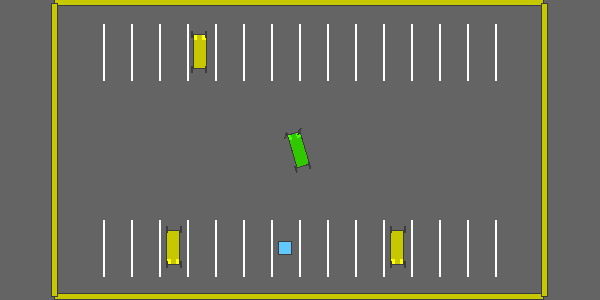
\includegraphics[width=0.45\textwidth]{./pics/parking.jpg}
    \caption{The parking lot environment \texttt{empty} with 0 other vehicles. The ego-vehicle is the green one, other vehicles are yellow, and the parking spot is the blue rectangle. There are walls on each side of the parking lot.}
    \label{fig:parking_lot}
\end{figure}

Note that the \texttt{highway-env} environment follows the OpenAI Gym API and configurations are stored in a YAML file where we can specify the action, observation, reward, vehicle number, has walls or not, and other settings. To make a gif output, \texttt{offscreen-rendering} should be unenabled.

\subsection{Reinforcement Learning algorithms}

The reason for adopting reinforcement learning (RL) algorithms in this project is that the autonomous parking task is a sequential decision-making problem with a continuous action space, where optimal strategies must be learned through interactions with the environment. RL algorithms are well-suited for such problems due to their ability to handle complex dynamics, perform long-term planning, and optimize policies without requiring expert demonstrations. This project utilizes the Stable-Baselines3 \cite{stable-baselines3} library to implement three widely used RL algorithms: Twin Delayed DDPG (TD3) \cite{fujimoto2018addressing}, Soft Actor-Critic (SAC) \cite{haarnoja2018soft}, and Proximal Policy Optimization (PPO) \cite{schulman2017proximal}. These algorithms are particularly effective for continuous control tasks. A brief overview of each is provided below.

\textbf{TD3} is and off-policy actor-critic algorithm that builds on the DDPG algorithm by introducing several improvements: target policy smoothing, delayed policy updates, and twin Q-networks to reduce the problem of overestimation bias. These enhancements make TD3 more stable, data-efficient, and accurate than DDPG, especially in environments with high-dimensional action spaces. However, TD3 requires careful hyperparameter tuning and deterministic policies could be less robust in stochastic settings.

\textbf{SAC} is an off-policy algorithm that improves a stochastic policy by maximizing entropy in addition to the expected return (i.e., exploration). This encourages a strong sample efficiency, more balanced exploration and exploitation, and higher tolerance to environment noise. Meanwhile, SAC has a relative high computational cost and also requires careful hyperparameter tuning on entropy coefficient and learning rates.

\textbf{PPO} is an on-policy policy gradient method that uses a clipped surrogate objective to optimize the policy. It is a simple yet stable and effective algorithm in many continuous control tasks. However, the on-policy nature makes it less sample-efficient and may perform suboptimally in high dimensional action spaces.

\subsection{Observation, Reward Function and Training Settings}

Usually, the training settings of RL algorithms are highly influence the performance of the agent and transferability to real-world scenarios. This subsection first describes the observation modalities, followed by the reward function and other training settings.

\textbf{Observation Modalities.} The \texttt{highway-env} environment naturely supports all the three sensing modalities we need: Vision (GrayScale Image), Radar (Kinematics), and LiDAR, where in the parentheses are the names used by the \texttt{highway-env}.

\begin{enumerate}
  \item \textbf{Vision (GrayScale Image):} The observation is a $W \times H$ image, where $W$ and $H$ are configurable parameters. Several images can be stacked to enable the agent to perceive dynamic changes without explicit memory.
  \item \textbf{Radar (Kinematics):} The observation is a $V \times F$ array, where $V$ is the number of vehicles in the environment and $F$ is the number of features (e.g., position, velocity, acceleration, etc.). Options include normalization and using absolute positions.
  \item \textbf{LiDAR:} The observation is a $N \times 2$ array, where $N$ is the number of divided angular sectors around the ego-vehicle. For each sector, 1) the distance to the nearest collidable object and 2) the relative velocity along that direction are recorded. Configurable parameters include normalization, number of sectors, and maximum detectable distance. Figure~\ref{fig:lidar} illustrates the LiDAR observation.
\end{enumerate}

\begin{figure}[h]
    \centering
    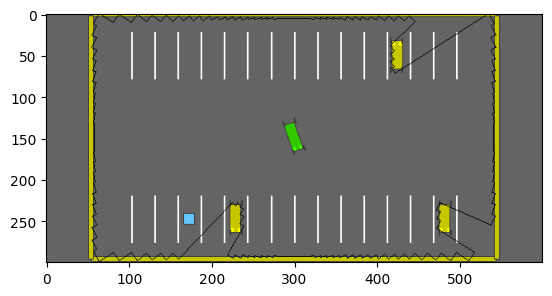
\includegraphics[width=0.45\textwidth]{./pics/lidar.png}
    \caption{The LiDAR observation.}
    \label{fig:lidar}
\end{figure}

\textbf{Reward Function.} The reward function is crucial for guiding the agent to learn the desired behavior. In this project, the reward function is designed to encourage parking while penalizing collisions and deadlocks, which remains the default setting as environment provided. The reward function is defined as follows:

\begin{align*}
    \mathbf{s} &= [x, y, v_x, v_y, \cos(h), \sin(h)]^T \\
    \mathbf{w} &= [1, 0.3, 0, 0, 0.02, 0.02]^T \\
    R_{\text{total}} &= (\mathbf{w}^T \mathbf{s}) - 5 \cdot \mathbb{I}(\text{collision}) + 0.12 \cdot \mathbb{I}(\text{success})
\end{align*}

where $\mathbf{w}^T \mathbf{s}$ reward the agent for moving towards the parking spot in a good direction, $- 5 \cdot \mathbb{I}(\text{collision})$ penalizes the agent for colliding, and $0.12 \cdot \mathbb{I}(\text{success})$ rewards the agent for successfully parking.

\textbf{Training Settings.} The training settings are summarized in Table~\ref{tab:training_settings}.

\begin{table}[h]
    \centering
    \begin{tabular}{l|c}
        \hline
        \textbf{Parameter} & \textbf{Value} \\
        \hline
        Action Space & Continuous (steering angle, acceleration) \\
        Observation Space & Varying by sensing modality (see above) \\
        Discount Factor ($\gamma$) & 0.99 \\
        Training Timesteps & 500,000 \\
        Batch Size & 256 \\
        Learning Rate & 0.001 \\
        Target Network Update Frequency (TD3/SAC) & 1,000\\
        Policy Update Frequency (TD3) & 2 \\
        Entropy Coefficient (SAC) & Auto-tuned \\
        Number of Vehicles in Environment & Varies by difficulty (0, 3, or 10) \\
        Parking Spot Size & Configurable (default: 2m x 5m) \\
        Maximum Detectable Distance (LiDAR) & Configurable (default: 50m) \\
        Number of LiDAR Sectors & Configurable (default: 36) \\
        Render Mode & RGB array for visualization and GIF \\
        \hline
    \end{tabular}
    \caption{Summary of training settings.}
    \label{tab:training_settings}
\end{table}

\section{Experiments 30\%}\label{sec:experiments}

This section presents the experimental results of the project, including ...

\section{Conclusion 5\%}\label{sec:conclusion}














\newpage

\section*{Acknowledgments}
The final project was independently conducted by the author Kunyi Yu. Meanwhile, the author would like to thank Professor Jiachen Li and TAs for their patient guidance and help.

\bibliographystyle{unsrtnat}
\bibliography{refs}

\appendix
\section*{Appendix}
\subsection*{How to Find the Code?}
The GitHub public repository for this project is at \url{https://github.com/Rock3Yu/EE245_Advanced_Robotics}. Please feel free to explore the code and data files. The structure of the repository is as follows:

\begin{verbatim}
./project
  |-- final
  |   |-- main.pdf
  |   |-- main.tex
  |   |-- ...
  |-- proposal
  |   |-- main.pdf
  |   |-- main.tex
  |   |-- ...
  |-- src
      |-- HighwayEnv
      |-- make_gif.py
      |-- models
      |-- parking_config.py
      |-- smallCNN.py
      |-- tensorboard_logs
      |-- train_0_kinematics.py
      |-- train_1_vision.py
      |-- train_2_lidar.py
      |-- ...
# The purpose of each dictory/file is as their name suggests.
\end{verbatim}

\end{document}